\documentclass{article}
\usepackage[nonatbib]{project}

\usepackage[breaklinks=true,letterpaper=true,colorlinks,citecolor=black,bookmarks=false]{hyperref}

\usepackage{amsthm}
\usepackage{amsmath,amssymb}
\usepackage{enumitem}
\usepackage{comment}

\usepackage[sort&compress,numbers]{natbib}
\usepackage[normalem]{ulem}

% use Times
\usepackage{times}
% For figures
\usepackage{graphicx} % more modern
%\usepackage{epsfig} % less modern
%\usepackage{subfig} 

\graphicspath{{../fig/}}

\usepackage{tikz}
\usepackage{tkz-tab}
\usepackage{caption} 
\usepackage{subcaption} 
\usetikzlibrary{shapes.geometric, arrows}
\tikzstyle{arrow} = [very thick,->,>=stealth]

\usepackage{cleveref}
\usepackage{setspace}
\usepackage{wrapfig}
%\usepackage[ruled]{algorithm}
\usepackage{algpseudocode}
\usepackage[noend,linesnumbered]{algorithm2e}

\usepackage{times}
\usepackage{latexsym}
\usepackage{graphicx}
\usepackage{amsfonts}
\usepackage{amsmath}
\usepackage{multirow}
\usepackage{booktabs}
\usepackage{makecell}
\usepackage{url}
\usepackage{float}

\usepackage[disable]{todonotes}

\newcommand{\red}[1]{\textcolor{red}{#1}}

\title{How does LSTM make Prediction? Contextual Decomposition for Rationalizing LSTM Predictions}

%\author{
%	Yuqing Xie \\
%	University of Waterloo\\
%	\And
%	Peng Shi\\
%	University of Waterloo\\
%}

\begin{document}
\maketitle
% expect the report to be less than \textbf{8 pages} (references excluded).

%TODO
% introduction refine
% related work, conclusion
% question 2 find examples to draw plot
% mask uni-bw data
% question 2 pattern extraction experiment 

\begin{abstract}

LSTMs are widely used in Natural Language Processing~(NLP) area and treated as contextual encoders, which are fundamental blocks of complicated models. Usually, LSTMs are regarded as black boxes and people contribute their effectiveness source to their context learning ability. In this paper, we are trying to understand the behaviors and rationalize the predictions of LSTMs. Based on Entity Detection task, we propose a token-level contextual decomposition method, to investigate the effectiveness sources of the LSTM models. With the help embedding visualization technique, we also show that embeddings also make a major contribution towards the model effectiveness.

\end{abstract}

\section{Introduction}

Long-Short-Term-Memory(LSTM) models are now the standard components to deal with natural language, achieving state-of-the-art performance on varieties of natural language tasks, ranging from machine translation~\cite{sutskever2014sequence}, question answering~\cite{tan2015lstm} to sentence classification~\cite{liu2016recurrent} and sentence tagging~\cite{chiu2016named}. However, unlike Convolution neural networks for vision tasks, the mechanism behind LSTM is less explored and hard to explain with visualization. Without clear understanding of the sequential models, further improvements are hard to make.

 Recently, some efforts have been made to try to understand LSTMs. \citet{strobelt2018lstmvis} and \citet{karpathy2015visualizing} analyzed the movement of the raw gate activations over a sequence. However, their cell co-ordinates based methods are usually hard to interpret and it is hard explain which inputs are important for specific outputs. On another line of research, derivative-based methods~\cite{alikaniotis2016automatic, denil2014extraction} are explored: by looking at the norm of the derivative of the loss function with respect to the embedding parameters for that word, they tried understand the model behavior in document classification. However, no exploration was made for token-level prediction tasks such as Entity Detection. 

Inspired by~\citet{murdoch2017automatic}, we propose a novel method of decomposing LSTM models on token level, to further understand their behaviors and predictions. The main difference between our work and \citet{murdoch2017automatic} is that they decompose the uni-directional LSTM on sentence level prediction, while we decompose the uni-directional LSTM and bi-directional LSTM on token level prediction. With our decomposition method, we can understand how do the tokens in a sentence influence the prediction of a specific token. This idea is quite similar to the attention mechanism in NLP~\cite{bahdanau2014neural}, which is usually used for explaining the predictions of the neural models. However, attention components will introduce extra parameters, and the original models are changed. Our decomposition method can be applied to any trained LSTM networks without any modification. 

With further experiments on Entity Detection task, we show that though Bi-LSTM indeed bring extra performance gains compared against uni-directional LSTMs or local models such as MLPs, word embedding still play an important role in predicting the results correctly. We also show several types of errors that the models make and analyze them with the help of the novel decomposition method. 

%However, no significant findings have been made to help understand the predictions on the token level. 
% TODO:related works summary.
%Why can't any of the existing techniques effectively tackle this problem?

% Since few theory work has been done to successfully dig deep into sequential models and apply the findings to practice, we proposed a novel method of decomposing Bi-LSTM models and visualize them for further model improvement. We decomposed trained Bi-LSTM models for sequence tagging tasks to understand the contribution of each components in the sentence. %We also improved the final model according to this finding. 
% take cross-view learning as an example in this project. We will analyze and improve cross-view learning using Bayesian ensemble.

% First thought to investigate the LSTM is to watch on the contribution of each word toward the output. A clear way to do this is to apply the attention mechanism. However, what we aim to do here is not to improve the model by introducing extra weights but to just examine the existing model. We follow Jame’s to decomposition[TODO]. The main idea is to decompose the output gates in LSTM and convert them in to the contribution weights of words towards outputs. Their work focus on the sentence classification tasks -- sentiment classification. This is relative simple task and needs less understanding of the sentence structure. Contributions of each word is relatively clear according to their meaning, which can be easily represented by current word embeddings. We follow their method  made modification of their models since we focus on sequence tagging tasks and examined Bi-LSTM.

%Possible difficulties - main contribution
%How to quantify the observations and summarize it into prior knowledge.
%How to integrate the human prior knowledge in Bayesian Ensemble.
%What properties did you analyze/prove about this problem or technique?

% \section{Related Works}

% There are mainly two lines of related work on neural network interpretability.

%TODO rewrite and summary.

% First, Hendrik et al. (2016) and Karpathy et al. (2016) analyze the movement of the raw gate activations over a sequence.
% Karpathy et al. (2016) is able to identify co-ordinates of $c_t$ that correspond to semantically meaningful attributes such as whether the text is in quotes and how far along the sentence a word is. However, most of the cell co-ordinates are harder to interpret, and in particular, it is often not obvious from their activations which inputs are important for specific outputs.

% Another approach that has emerged in the literature Alikaniotis et al. (2016) Denil et al. (2015) Bansal et al. (2016) is for each word in the document, looking at the norm of the derivative of the loss function with respect to the embedding parameters for that word. This bridges the gap between high-dimensional cell state and low-dimensional outputs. These techniques are general- they are applicable to visualizing the importance of sets of input coordinates to output coordinates of any differentiable function. In this work, we describe techniques that are designed around the structure of LSTM’s, and show that they can give better results in that setting.

%TODO
%Summarize the range of techniques by highlighting their strengths and weaknesses  differences or limitations (if any)? 
%Suggestion: organize your summary based on desirable properties of the techniques
%What is the state of the art?
%Any open problem?

\section{Models}

To understand the mechanism behind current sequential models, we follow [TODO Ian Tenney]'s ``edge probing'' framework to construct an architectures across tasks. Unlike [Tenney] focusing on sequence classification tasks, we focus on sequence tagging problem. That is to say, given a sentence, we have to give each token a label based on the whole sentence.

\subsection{Notations}
Formally, we represent a sentence as a list of tokens $T = [t_1, t_2, ... , t_n]$, where $n$ represents the length of the sentence, and the label of each token to be $L = [l_1, l_2, ... , l_n]$. Given a sequence of tokens, we embed the tokens into a high dimension vectors. Thus, a sentence can be represented as $E = [e_1, e_2, ... , e_n], e_i \in \mathbb{R}^d, \forall 1 \leq i \leq n$, where $d$ is the embedding size. Then we pass this embedded sentence into models.

%\red{We focus on the named entity recognition task. This is to tag each word its category in terms of entity, that is does the word refer to a person, a location, an organization, etc. Usually the system needs to tag for each token their category alone with whether it is the start, inner or end part of this entity. To make future analysis easier, we simplify the task to be a binary classification task. That is to say, we classify each token to be either entity or non-entity.} 
%states twice ?

We implement several models to compare the contribution of both embedding information and contextual information to the final prediction. 


\subsection{Uni-LSTM}

We follow the traditional LSTM mechanism to construct a model for sequence tagging task. Given a sequence of word embeddings, $E = [e_1, e_2, ... , e_n], e_i \in \mathbb{R}^d$, an Uni-LSTM processes one word at a time, keeping track of cell-gates $C = [c_1, c_2, ... , c_n]$ and hidden states $H = [h_1, h_2, ... , h_n]$. After processing each token, the hidden state of current token is then passed through a fully-connected layer to form the probability distribution over classes. After a softmax activation function and argmax, the model will predict a label across classes.

In detail, each Uni-LSTM cell computes $h_t$ and $c_t$ as a function of $e_t, c_{t-1}$ using the following updates. 
\begin{align} 
f_t & = \sigma(W_f x_t + V_f h_{t - 1} + b_f) \label{eq:1f}\\
i_t & = \sigma(W_i x_t + V_i h_{t - 1} + b_i) \label{eq:1i}\\
o_t & = \sigma(W_o x_t + V_o h_{t - 1} + b_o) \label{eq:1o}\\
\tilde{c}_t & = \tanh(W_c x_t + V_c h_{t - 1} + b_c) \\
c_t & = f_t \odot c_{t - 1} + i_t \odot \tilde{c}_t \label{eq:1c}\\
h_t & = o_t \odot \tanh(c_t)\label{eq:1h}
\end{align}

As initial values, we define $c_0=h_0=0$. 
Then the probability distribution for the $t$ th token for the $c$ th class is specified by 
\begin{equation}
p_{t, c} = \text{SoftMax}(W h_t + b) = \frac{e^{W_{:c} h_t + b_{:c}}}{\sum_{j = 1} ^ C e^{W_{:j} h_t + b_{:j}}},
\end{equation}
where $W_{:j}$ is the $i$ th row of the matrix $W$ and $b_{:j}$ is the bias of the $i$ th.

This is the forward LSTM. In this case, the information is passed from the beginning of the sentence to the end. We also consider the backward LSTM for later comparison. The only difference will be the update direction and the initial value. The initial values are assigned to $c_n=h_n=0$. And the information is passed from the end of the sentence to the beginning, which means we update the $t$ th token using the $t+1$ th token instead of the $t-1$ th as in the forward version.

\subsection{Bi-LSTM}

Uni-LSTM networks suffer from only seeing information from one side of t he sentence. So we also include a Bi-LSTM to examine the information learnt from both sides. The encoding process is just simply concatenate forward and backward gates together. We demote the forward gates as $f_t^{fw}, i_t^{fw}, o_t^{fw}, c_t^{fw}, h_t^{fw}$, and the backward gates as $f_t^{bw}, i_t^{bw}, o_t^{bw}, c_t^{bw}, h_t^{bw}$. We also demote the concatenated matrix of $*_t^{fw}$ and $*_t^{bw}$ as $[*_t^{fw}, *_t^{bw}]$. After concatenate the forward and backward gates together, using $[*_t^{bw}, *_t^{fw}]$ to replace $*_t$ in formulas from \ref{eq:1f} to \ref{eq:1h}, we can represent the update formulas in a same form. 

Also probability distribution for the $t$ th token for the $c$ th class is specified by 
\begin{equation}
p_{t, c} = \text{SoftMax}(W [h_t^{fw}, h_t^{bw}] + b) = \frac{e^{W_{:c} [h_t^{fw}, h_t^{bw}] + b_{:c}}}{\sum_{j = 1} ^ C e^{W_{:j} [h_t^{fw}, h_t^{bw}] + b_{:j}}}.
\end{equation}

\subsection{MLP}

To examine what information has been learnt by LSTM from the context and what information can be directly learned from the word embedding, we also implemented a m-layer MLP network to tag the tokens only according to the embeddings. Each MLP layer can be represented as follow:
The input of the $i$ th layer is represented as $x_i$, then the $i$ th layer is $f_i(x_i) = \sigma(W_i x_i + b_i)$, where $W_i$ and $b_i$ are the weights and bias of the $i$ th layer. In this work we use ReLU as our activation function $\sigma$. Then the output of the $i$ th layer $f_i(x_i)$ is then feed into the next layer as input. That is to say $x_{i+1} = f_i(x_i)$. 

We compared the four different embeddings: the original pre-trained embedding from GloVe, the tuned embedding of forward and backward Uni-LSTM and the Bi-LSTM. The final probability will be $p_{t, c} = \text{SoftMax}(f_m(e_t))$.% explain more?

\subsection{Uni-LSTM Decomposition}
\label{uni-lstm-decom}

We now show that we can decompose the numerator of $p_{t, c}$ into a product of factors, and interpret those factors as the contribution of individual words of the predicted probability of class $c$ for Uni-LSTM. Also taking the forward direction as an example, define 
\begin{equation}\label{eq:uni-beta} 
\beta_{t, c, j} = \exp\left(W_{:c} (o_t \odot (\tanh(c_j)- \tanh(c_{j-1}))\right),
\end{equation}
so that 
\[\exp( W_{:c} h_t) = \exp\left(\sum_{j=1}^t W_{:c} (o_t \odot (\tanh(c_j) - \tanh(c_{j-1}))\right) = \prod_{j=1}^t \beta_{t, c, j}.\]

As $\tanh(c_j) - \tanh(c_{j-1})$ can be viewed as the update resulting from word $j$, so $\beta_{t, c, j}$ can be interpreted as the multiplicative contribution to $p_{t, c}$ by word $j$. 

Now, we have 
\begin{equation}
p_{t, c} \propto \exp( W_{:c} h_t + b_{:c}) = \exp(b_{:c})\prod_{j=1}^t \beta_{t, c, j}.
\end{equation}

This is a direct extension of [TODO]'s work, in which we expand their method to suit sequence tagging tasks.
The backward direction will just be the same.

\subsection{Bi-LSTM Decomposition}
\label{bi-lstm-decom}

We also extend the decomposition for Bi-LSTM model. For Bi-LSTM, we can simply de-concatenate the gate states and compute the contribution of each direction as in the Uni-LSTM. Then each token's probability distribution can be taken as a combination of both direction. That is to say, the probability can be interpreted as follow:
\begin{align}\label{eq:bi-beta} 
\beta_{t, c, j} = \exp(&W_{:c} [h_t^{fw}, h_t^{bw}])\\
= \exp(&W_{:c}^{fw} (o_t^{fw} \odot (\tanh(c_j^{fw})- \tanh(c_{j-1}^{fw}))) \\
+ &W_{:c}^{bw} (o_t^{bw} \odot (\tanh(c_j^{bw})- \tanh(c_{j+1}^{bw})))),
\end{align}
Let
\begin{equation}
\beta_{t, c, j}^{fw} = \exp(W_{:c}^{fw} (o_t^{fw} \odot (\tanh(c_j^{fw})- \tanh(c_{j-1}^{fw}))))
\end{equation}
and
\begin{equation}
\beta_{t, c, j}^{bw} = \exp(W_{:c}^{bw} (o_t^{bw} \odot (\tanh(c_j^{bw})- \tanh(c_{j+1}^{bw}))))
\end{equation}
so that 
\begin{equation}
\beta_{t, c, j} = \beta_{t, c, j}^{fw} \beta_{t, c, j}^{bw}
\end{equation}
Then we have:
\begin{align}
p_{t, c} \propto \exp(&W_{:c} [h_t^{fw}, h_t^{bw}] + b_{:c}) \\
= \exp(&b_{:c} + \sum_{j=1}^t W_{:c}^{fw} (o_t^{fw} \odot (\tanh(c_j^{fw}) - \tanh(c_{j-1}^{fw})))\\
	+&\sum_{j=t}^n W_{:c}^{bw} (o_t^{bw} \odot (\tanh(c_j^{bw}) - \tanh(c_{j+1}^{fw}))))\\
=  \exp(&b_{:c})\prod_{j=1}^t \beta_{t, c, j}^{fw} \prod_{j=t}^n \beta_{t, c, j}^{bw}.
\end{align}

\section{Model Comparison} \label{sec:question}

For better understanding, we break down the problem of ``What does the Bi-LSTM learn'' into three small problems:

\begin{itemize}
	\item Do Bi-LSTM perform significantly better than Uni-LSTM and local models such as MLP? 
	In what cases, each model works well?
	\item Why do Uni-LSTM and local model work in some cases? 
	\item How LSTMs make their prediction? How do they make errors? Why do they have better performance?% Does Bi-LSTM model learn to do prediction from contextual information? How to verify and measure the difference? 
\end{itemize}

To answer first question, we conduct the experiments with Bi-LSTM, Uni-LSTM model. The embedding is initialized with GloVe pretrained embeddings~\cite{pennington2014glove}. To investigate what kind of information gain provided by the LSTM, we also conduct experiments with MLP. We adopt the fine-tuned embeddings in LSTM and fix them during the training of MLP model. This is known as probing technique. 

To answer the second question, we leverage visualization techniques such as t-SNE~\cite{maaten2008visualizing}, to visualize embedding vectors. T-SNE is a technique that can visualizes high-dimensional data by giving each datapoint a location in a two or three-dimensional map. The main idea is to first use mixture models to estimate the distribution of points and then minimize the KL-divergence between point distributions before and after the mapping.

To answer the third question, we use the LSTM decomposition technique to further investigate the contribution distribution for the token level prediction. The decomposition is conducted for Bi-LSTM and Uni-LSTM. 

\section{Experimental Setup}

%We conduct extensive experiments to answer the question: What do the Bi-LSTM learn? 

\subsection{Dataset} 

Our experiments are conducted on OntoNotes 5 English dataset~\cite{weischedel2012ontonotes}, focusing on Entity Detection task. The Entity Detection task is usually formulated as a sequence labeling task: labels are assigned to each token. Different tagging scheme can be adopted, such as \textit{BIO}, \textit{BIOES}, etc. For simplification, in this work, we use \textit{IO} scheme: if the token is a part of entity, it will be annotated as \textbf{I}; otherwise, it will be annotated as \textbf{O}. One special case that this tagging scheme can not handle is that two entity appear consecutively in one sentence, because there is not boundary label such \textbf{B}~(begin of entity). So in our experiments, we remove the sentences with consecutive entities for further experiments. The performance is evaluated by Precision, Recall and F1 scores.

\subsection{Hyper-parameters}


\section{Results}

We demonstrate our results regarding questions in Section \ref{sec:question}. Here, Uni-LSTM-forward denotes forward Uni-directional LSTM; Uni-LSTM-backward has similar meanings. MLP(GloVe) denotes the MLP model trained with GloVe embeddings which are finetuned during the learning on Entity Detection task. MLP(bi) denotes the MLP model based on the tuned embeddings from Bi-LSTM model. The embedding is fixed and we only tune the perceptron weights. MLP(uni-forward) and MLP(uni-backward) have similar meanings.

\subsection{Bi-LSTM is better.}

\begin{table}[t]
	\centering
	\begin{tabular}{l@{\qquad}ccc}
		\toprule
		\textbf{Model}         & \textbf{Precision} & \textbf{Recall} & \textbf{F1} \\ \midrule
		Bi-LSTM &  84.82 & 83.60  & 84.20 \\
		Uni-LSTM-forward & 72.47 & 73.88 & 73.17 \\
		Uni-LSTM-backward & 80.31 & 80.28 & 80.29 \\ \midrule
		MLP(GloVe) & 60.63 & 61.82 & 61.22 \\
		MLP(bi) & 54.97 & 75.65 & 63.67 \\ 
		MLP(uni-forward) & 60.80 & 61.75 &  61.27 \\ 
		MLP(uni-backward) & 54.61 & 75.99 & 63.55 \\ 
		\bottomrule
	\end{tabular}
	\vspace{3mm}
	\caption{Entity Detection performance on OntoNotes 5 English Dataset Test set. }
	\label{res:ner}
\end{table}

The Table~\ref{res:ner} shows the experiment results of effectiveness models. 
We can observe that Bi-LSTM has better F1 score~(+11.03) than Uni-LSTM, which is a large gap in the Entity Detection task. However, we can observe that Uni-LSTM-backward performs significantly better than Uni-LSTM-forward, with large margin~(+7.12), and approaching the effectiveness of Bi-LSTM.

For the group of MLP models, we can find that they have similar performance~(around 60 F1 scores). Using the embeddings learned from the LSTM models does not provide much gains on the effectiveness comparing to MLP(GloVe). 
%Further comparing the results of Bi-LSTM and MLP(bi), we can better understand the gains brought by the Bi-LSTM contextual encoding layer. 
%Even leveraging the embeddings learned in Bi-LSTM model, the fine-tune MLP model still falls far behind the Bi-LSTM model. 
This comparison proves that the Bi-LSTM indeed empowers the entity detection ability. 

In order to quantify the errors that Uni-LSTM or MLP makes, we conduct further error analysis. We select examples that Bi-LSTM makes correct predictions and but Uni-LSTM or MLP fails, and further categorize them into 4 types, as discussed below.
And the detailed statistics is shown in Table~\ref{res:ner_error}. 

\begin{itemize}
	\item \textbf{Type A}: Wrongly predicting in-vocabulary words as entity. For example,\textit{ For \textbf{more} information check out : www.taconet.com.tw/cstudio/.} The model falsely predicts \textbf{more} as entity.
	\item \textbf{Type B}: Wrongly predicting out-of-vocabulary words as entity. For example, \textit{Another popular technique involves covering the trees with black \textbf{mosquito} nets to improve yields.} The model falsely predicts \textbf{mosquito} as entity while it is an out-of-vocabulary word.
	\item \textbf{Type C}: Failed to predict in-vocabulary words as entity. For example, \textit{Qichen Qian expressed welcome over the visit by vice \textbf{Foreign} Affairs Minister Kamyao and the political consultations in progress}. The model miss to predict an in-vocabulary word \textit{Foreign} as a part of entity.
	\item \textbf{Type D}: Failed to predict out-of-vocabulary words as entity. For example, \textit{\textbf{Guofang} Shen said that this bill is a bill carrying political discrimination and extremely unfriendly to China}. The model miss to predict an out-of-vocabulary word \textbf{Guofang} as a part of entity.
\end{itemize}

\begin{table}[t]
	\centering
	\begin{tabular}{l@{\qquad}cccc}
		\toprule
		\textbf{Model}         & Type A & Type B & Type C & Type D \\ \midrule
		uni-LSTM-forward &  239  & 117 & 823 & 214 \\
		uni-LSTM-backward & 191 & 97 & 214 & 256  \\
		MLP(bi) & 418 & 1675 & 1363 & 0  \\ 
		\bottomrule
	\end{tabular}
	\vspace{3mm}
	\caption{Error Analysis }
	\label{res:ner_error}
\end{table}

\begin{table}[t]
\small
\centering\centering\resizebox{\columnwidth}{!}{
\begin{tabular}{llp{7cm}}
\toprule
\textbf{Category}	& \textbf{Counts}	&\textbf{Examples} \\ \midrule

\textbf{Capitalization}					& 2		& \textbf{Thick} fog , rain and high winds are limiting visibility at the site .  \\
\textbf{OOV}					& 11		& Even if you wanted to , you wo n't be reading \textbf{Jermaine} 's account now.\\
\textbf{Missing Context	}		& 51		&Ah , yes , something called \textbf{a} Star Chamber .\\
\textbf{Others}  		& 9		&  - \\%And although Pennsylvania and Massachusetts suffered slight declines \textbf{earlier} in the decade , they are growing again .\\
\bottomrule
\end{tabular}}
\vspace{3mm}
\caption{Statistic of error source of Uni-LSTM(forward) model.}
\label{tab:bi-uni}
\end{table}

\begin{table}[t]
	\small
	\centering\centering\resizebox{\columnwidth}{!}{
		\begin{tabular}{llp{7cm}}
			\toprule
			\textbf{Category}	& \textbf{Counts}	&\textbf{Examples} \\ \midrule
			
			\textbf{Capitalization}	&13		&  \textbf{Consumer} activists are skeptical. \\
			\textbf{OOV}	& 46		& I forced myself to refrain from the grief of \textbf{loosing} my beloved car -LRB- mine was liability - only coverage -RRB- and asked the friend to send their family home.\\
			\textbf{Missing Context }	& 20		& It says that what \textbf{the} North Koreans did was a threat to international peace and security.\\
			\textbf{Others}	& 16		&  - \\% It achieved a total volume of 4 billion US dollars of goods going into and out of the area , increasing by 83 \% over \textbf{the same period of the previous} year , with a total amount of 1 billion US dollars from imports and exports.\\
			\bottomrule
	\end{tabular}}
	\vspace{3mm}
	\caption{The statistics of error source of MLP(bi) model.}
	\label{tab:bi-mlp}
\end{table}

To further examine the error sources, we also sample 50 sentences from the pool where Bi-LSTM makes correct predictions while uni-LSTM-forward makes wrong predictions. For MLP model, we also sample 50 sentences for error source analysis. We categorize the error sources into 4 types, as shown below.

\begin{itemize}
	\item \textbf{Capitalization}: Since GloVe embedding is case-sensitive, lowercased words and capitalized words have different embedding vectors, which lead to different inference. 
	\item \textbf{OOV}: Out of vocabulary~(OOV) words will be replaced by $<$UNK$>$ and then inference will be totally determined by the context. The models fail in some cases to infer that word as a part of entity.
	\item \textbf{Missing Context} The model fails to classify an in-vocabulary word as a part of entity because the model ignores the contextual information. 
	\item \textbf{Other} Other error sources which are hard to determined are classified into this category.
\end{itemize}

The counts of each categories and their examples are shown in Table~\ref{tab:bi-uni} and Table~\ref{tab:bi-mlp}. Note that one sentence might have more than one errors so the sum of the counts are larger than 50.

\subsection{Word Embedding and context both contributes to prediction.}

\noindent \textbf{A Motivating Example} 

To examine the source of effectiveness of LSTM, we conduct an experiment where the entities are randomly masked in test set. To eliminate the effect of word embedding and to measure the contribution from context, we mask the entities to $<$UNK$>$. The results are shown in \ref{tab:mask}.

\begin{table}[t]
	\centering
	\begin{tabular}{l@{\qquad}ccc}
		\toprule
		\textbf{Model}		& \textbf{Precision}	& \textbf{Recall}	& \textbf{F1} \\ \midrule
		Bi-LSTM-masked 	& 64.53~(-20.29) 			& 33.74~(49.86)			& 44.31~(-39.89) \\ 
		Uni-LSTM-forward-masked & 67.01~(-5.46) 		& 27.98~(-45.90) 			& 39.48~(-33.69) \\ 
		Uni-LSTM-backward-masked& 65.54~(-14.77) 		& 25.90~(-54.38)			& 37.12~(-43.17) \\ 
		\bottomrule
	\end{tabular}
	\vspace{3mm}
	\caption{Entity Detection performance on masked OntoNotes 5 English Dataset Test set. The numbers in bracket denote the performance degradation compared with the corresponding models.}
	\label{tab:mask}
\end{table}

We can find that the recall drop dramatically after masking the entities to $<$UNK$>$. This means the models fail to detect entities without embedding information from the words themselves. This give us the idea that effectiveness of sequence tagging may mainly come from the word embedding. So we analysis the embedding using visualization techniques.

\noindent \textbf{Analysis}

\begin{figure}[t]
	\centering
	\begin{subfigure}[t]{0.24\textwidth}
		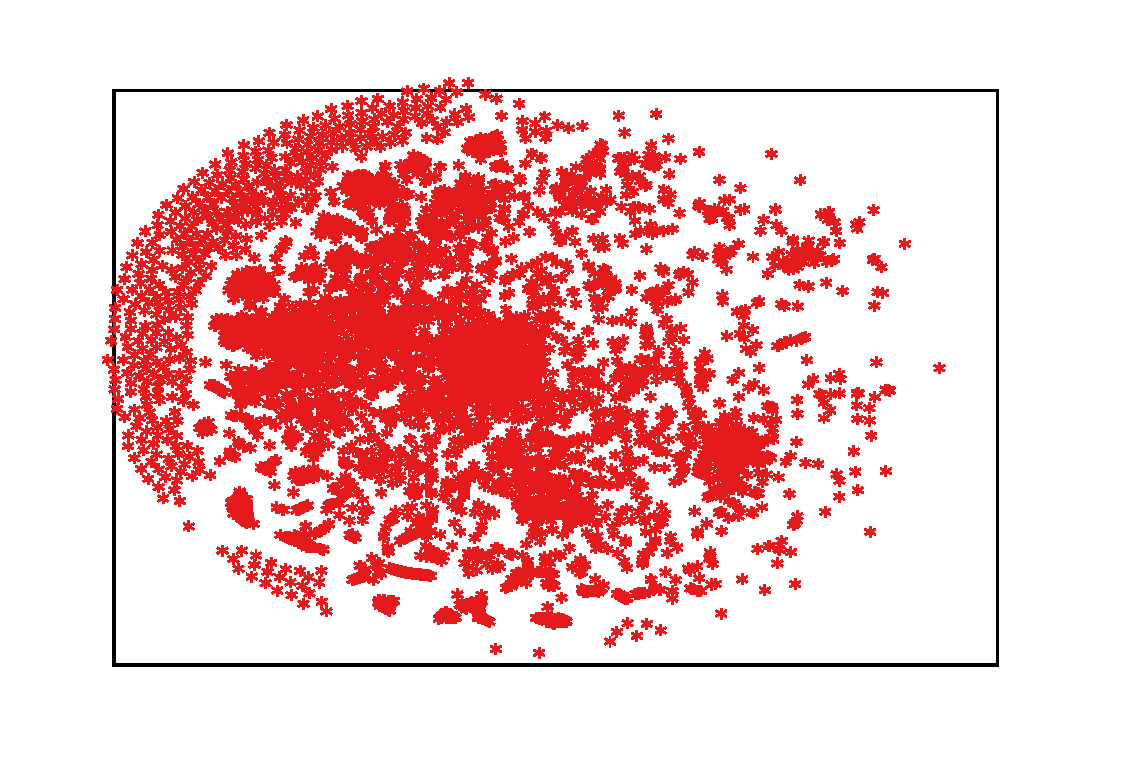
\includegraphics[width=\linewidth]{glove_embedding_positive_mirror.pdf}
		\caption{GloVe Embedding with entity word}
		\label{fig:glove_positive}
	\end{subfigure} \hfil 
	\begin{subfigure}[t]{0.24\textwidth}
		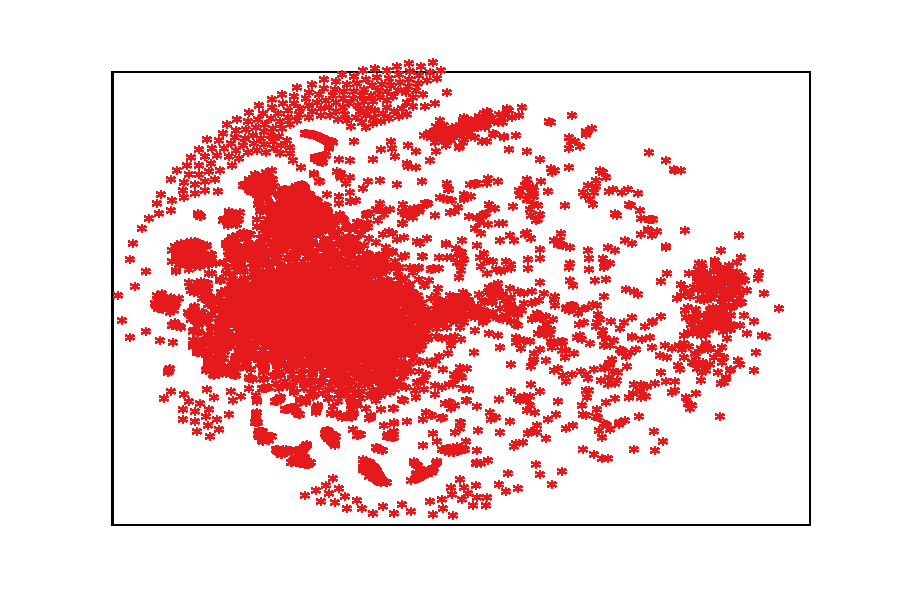
\includegraphics[width=\linewidth]{bi_lstm_gold_positive.pdf}
		\caption{Bi-LSTM Embedding with entity word}
		\label{fig:bi_lstm_gold_positive}
	\end{subfigure} \hfil 
	 \begin{subfigure}[t]{0.24\textwidth}
		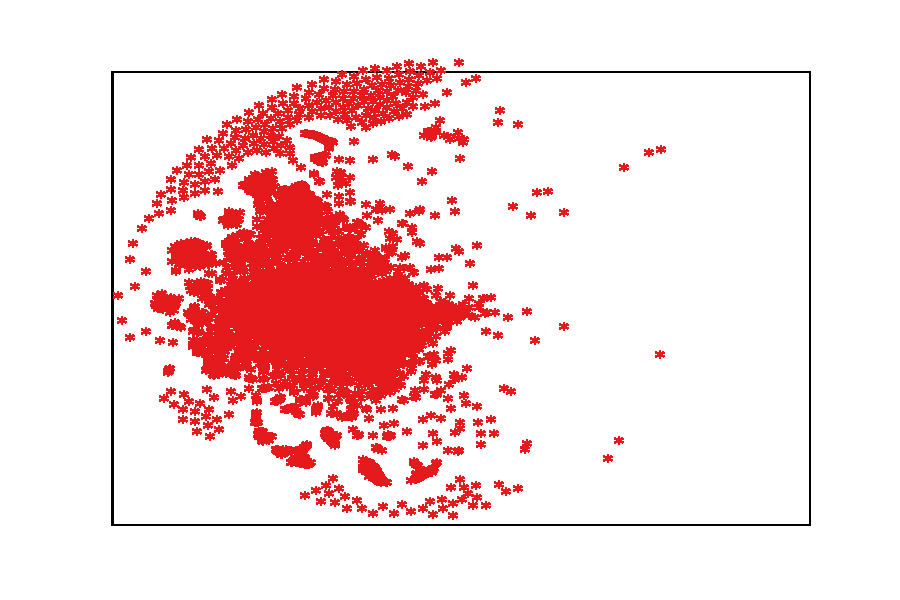
\includegraphics[width=\linewidth]{bi_lstm_mlp_positive.pdf}
		\caption{Bi-LSTM Embedding with entity word based on the prediction of MLP model}
		\label{fig:bi_lstm_mlp_positive}
	\end{subfigure}

	\bigskip
	
	\begin{subfigure}[t]{0.24\textwidth}
		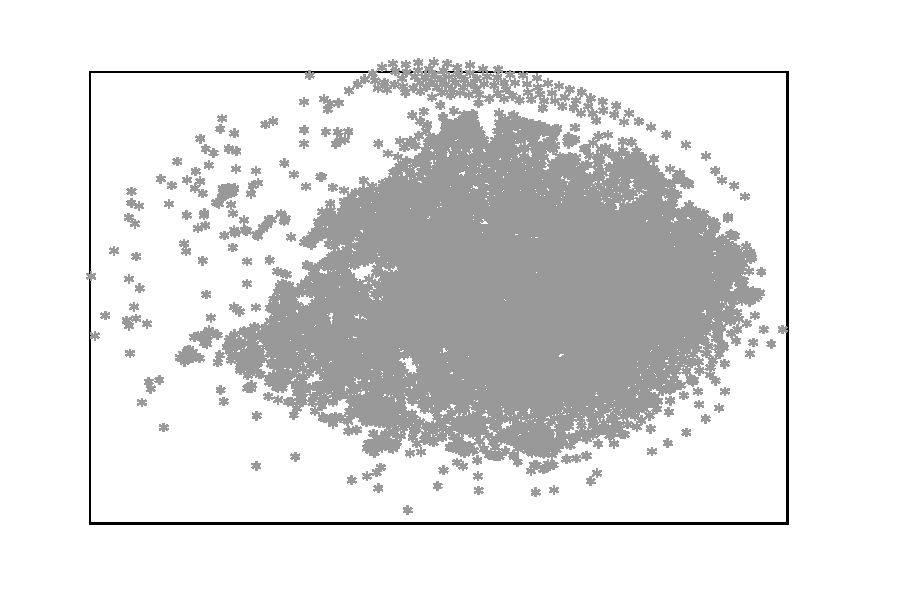
\includegraphics[width=\linewidth]{glove_embedding_negative_mirror.pdf}
		\caption{GloVe Embedding with non-entity word}
		\label{fig:glove_negative}
	\end{subfigure} \hfil
   \begin{subfigure}[t]{0.24\textwidth}
	   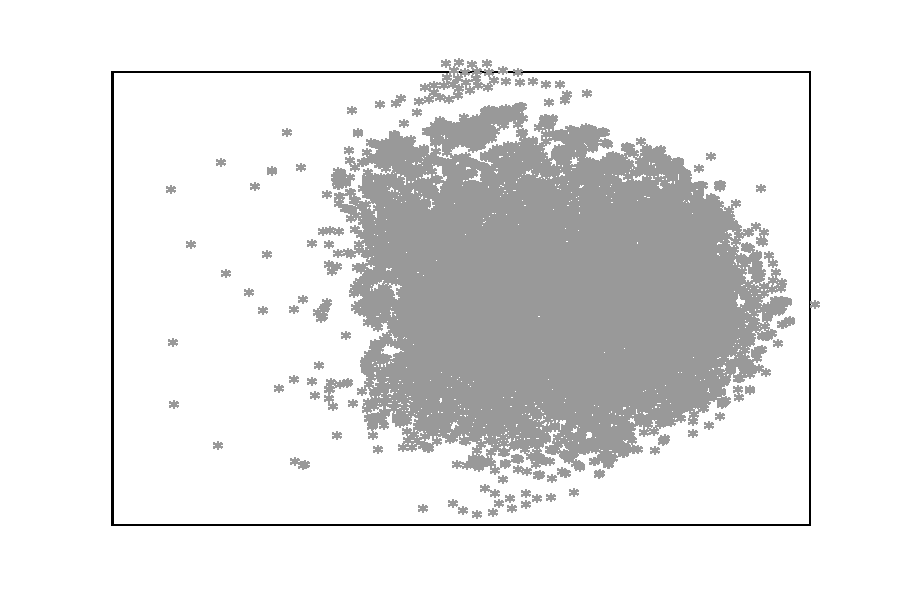
\includegraphics[width=\linewidth]{bi_lstm_gold_negative.pdf}
	   \caption{Bi-LSTM Embedding with non-entity word}
	   \label{fig:bi_lstm_gold_negative}
   \end{subfigure} \hfil
	\begin{subfigure}[t]{0.24\textwidth}
		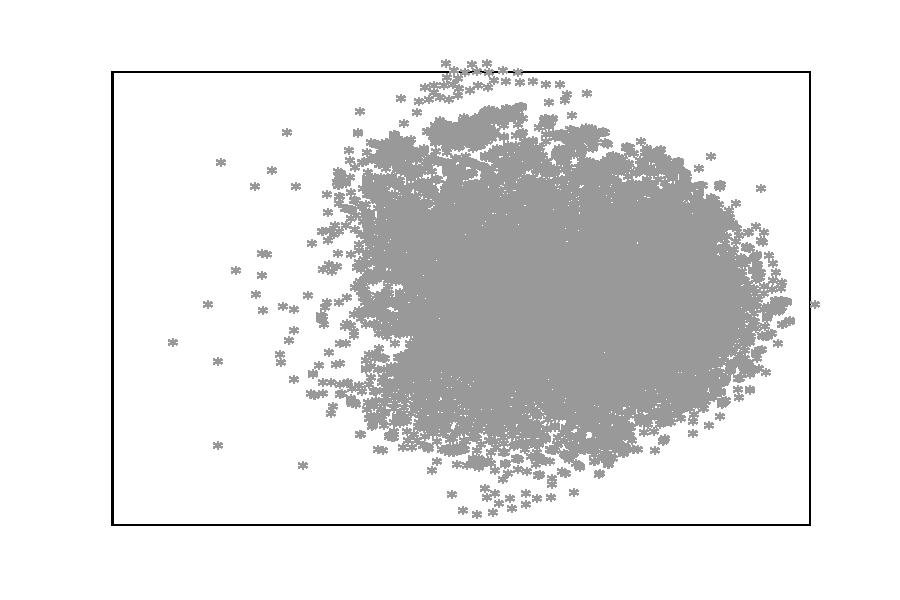
\includegraphics[width=\linewidth]{bi_lstm_mlp_negative.pdf}
		\caption{Bi-LSTM Embedding with non-entity word based on the prediction of MLP model}
		\label{fig:bi_lstm_mlp_negative}
	\end{subfigure}
	\caption{T-SNE for Word Embedding}
	\label{fig:embedding}
\end{figure}

We can observe that with local model such as MLP, the model can achieve reasonable performance. More than 60 F1 score can be obtained by simple local model, as shown in Table~\ref{res:ner}. %In this subsection, we are trying to investigate the reason behind this, mainly focusing on the embedding level. 

To investigate the underlying rationals, we conduct the following analysis: we firstly classify the words into two categories: words belong to at least one entity~(entity word), and words nerve belong to any entity~(non-entity word). Then we leverage the t-SNE to decompose the embedding vectors into two dimensions and visualize them. In \ref{fig:embedding}, red dots denote entity words and grey dots denote non-entity words. 

Here, we decompose two sets of embeddings: original GloVe embeddings, embeddings learned from the Bi-LSTM.

The decomposition of the original GloVe embedding is shown in Figure~\ref{fig:glove_positive} and Figure~\ref{fig:glove_negative}. With these two figures, we can find that the GloVe embeddings indeed contain some entity-related information: the entity-words somehow group in the left side and non-entity-words distribute on the right side. But we still can find that a large amount of the entity and non-entity words are mixed in the middle of the figure. 

We further decompose the embeddings learned from the Bi-LSTM model, as shown in Figure~\ref{fig:bi_lstm_gold_positive} and Figure~\ref{fig:bi_lstm_gold_negative}. Compared with the figures from GloVe embeddings, we can observe that the entity-words are clustered tighter in Bi-LSTM based embeddings. This phenomenon indicates that the training process optimize the embeddings representation.

Based on the decomposition of learned Bi-LSTM embeddings, we assign each dot with the color based on the MLP(bi) predictions. In Figure~\ref{fig:bi_lstm_mlp_positive} and Figure~\ref{fig:bi_lstm_mlp_negative}, if MLP(bi) predict a word as a part of entity, then the corresponding dot will be colored with red; otherwise grey. Statistics tell us 84.95\% of the entity-words are correctly colored red by MLP(bi). This proves that the idea that the embeddings indeed contribute significantly on Named Entity Detection task.

% In question 1, we have empirically shown that the LSTM model could perform significantly better than local model, then we also want to show this in more deeper way. With LSTM decomposition, we find that the Bi-LSTM can correct several errors made by local model such as MLP and uni-LSTM. 

\noindent \textbf{Decomposition}

As discussed in Section~\ref{uni-lstm-decom} and Section~\ref{bi-lstm-decom}, we can decompose the LSTM to get contributions from other tokens to current token's prediction. We show several examples here to illustrate the process. We take $\log$ to $\beta_{t,j,c}$ for better visualization.

The first example is the contribution of each word to the word ``\textbf{Bill}'' in sentence \textit{``Let me conclude with comments by \textbf{Bill} the editor of Weekly Standard''}. It is an entity in under this case. 
\begin{figure}[t]
	\centering
	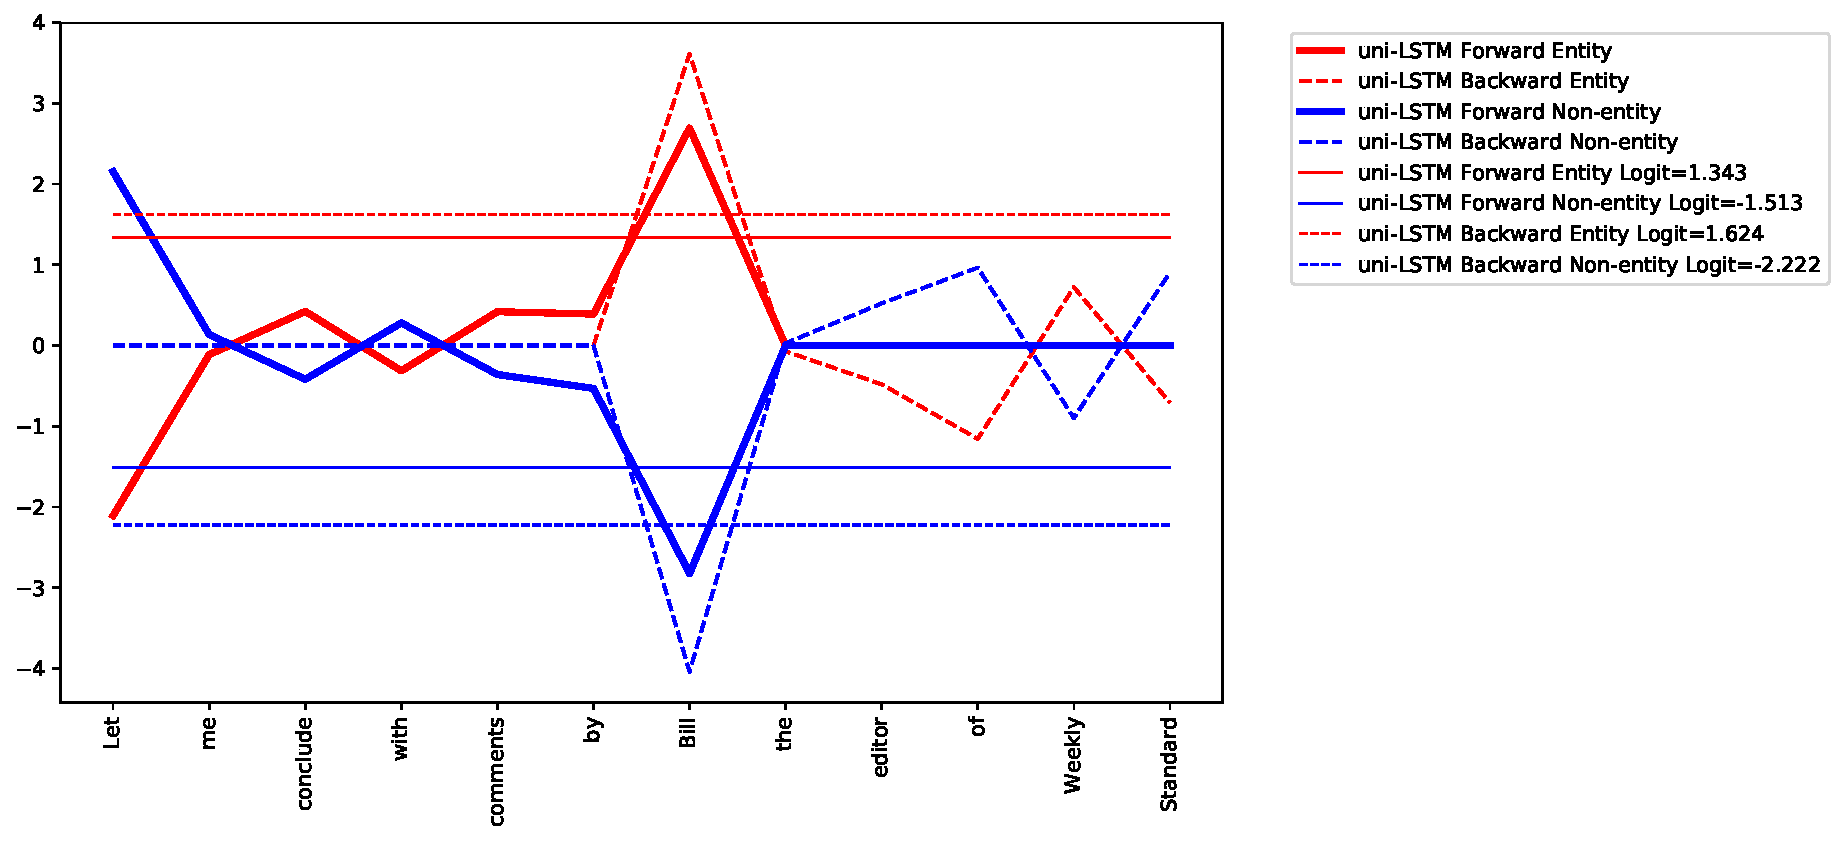
\includegraphics[width=\linewidth]{uni-Bill1.pdf}
	\caption{Example 1 for LSTM decomposition contributions to ``Bill''. The x-axis represents token id $j$, and the y-axis represents $\log \beta_{t, j, c}$}
	\label{fig:Bill}
\end{figure}

The solid lines represents the forward model's contribution while the dotted line represents the backward model's contribution.  Red lines represents the contribution to predict the target to be an entity while blue lines represents the contribution to predict the target to be a non-entity. We also add level lines to indicate the logits, which equal to $b_{:c} + \sum_{j=0}^{i} \log \beta_{i, j, c} $ for each class $c$.

As we can see from Figure~\ref{fig:Bill}, the contribution to two different classes are nearly symmetric. This makes sense because this is a binary-classification problem. Then we can find the main contribution to label \textbf{Bill} as an entity is from the word itself. The reason is also clear: ``Bill'' looks like a person's name because it's capitalized, so the entity information is already encoded in the word embedding vector. 

To eliminate the contribution from the word embedding, we change ``Bill'' in to ``bill''. In this case, we human can still recognize it as a person's name but just mis-capitalizing. In this case, the word ``bill'' is usually a common word represents non-entity so the embedding information will no longer tell the model that it is an entity.

\begin{figure}[t]
	\centering
	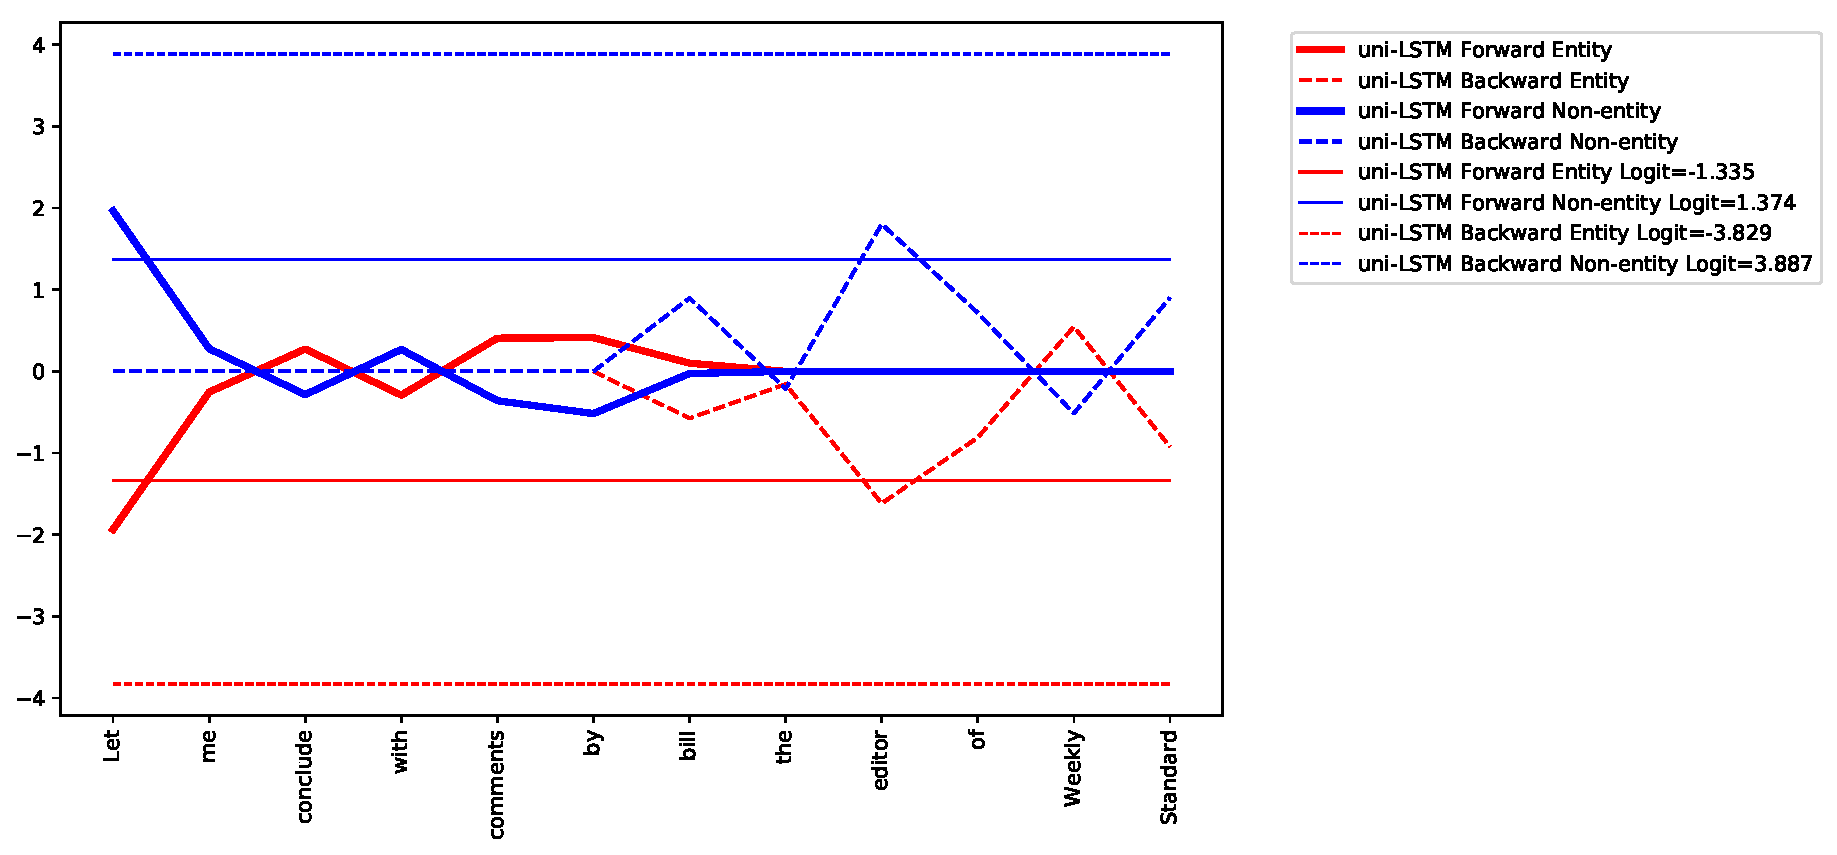
\includegraphics[width=\linewidth]{uni-bill2.pdf}
	\caption{Example 2 for LSTM decomposition contributions to ``bill''. The x-axis represents token id $j$, and the y-axis represents $\log \beta_{t, j, c}$}
	\label{fig:bill}
\end{figure}

Now, after the changing, we can see that the contribution from ``bill'' itself has decreased. So in this case, the Uni-LSTM mistakenly predict it as a non-entity. However, the ``bill'' is a less-entitish word, which may mislead the model to a wrong prediction. 

So to truely eliminate the contribution from the word embedding and focus more on the contextual information, we substitute ``Bill'' with ``$<$UNK$>$''.

\begin{figure}[t]
	\centering
	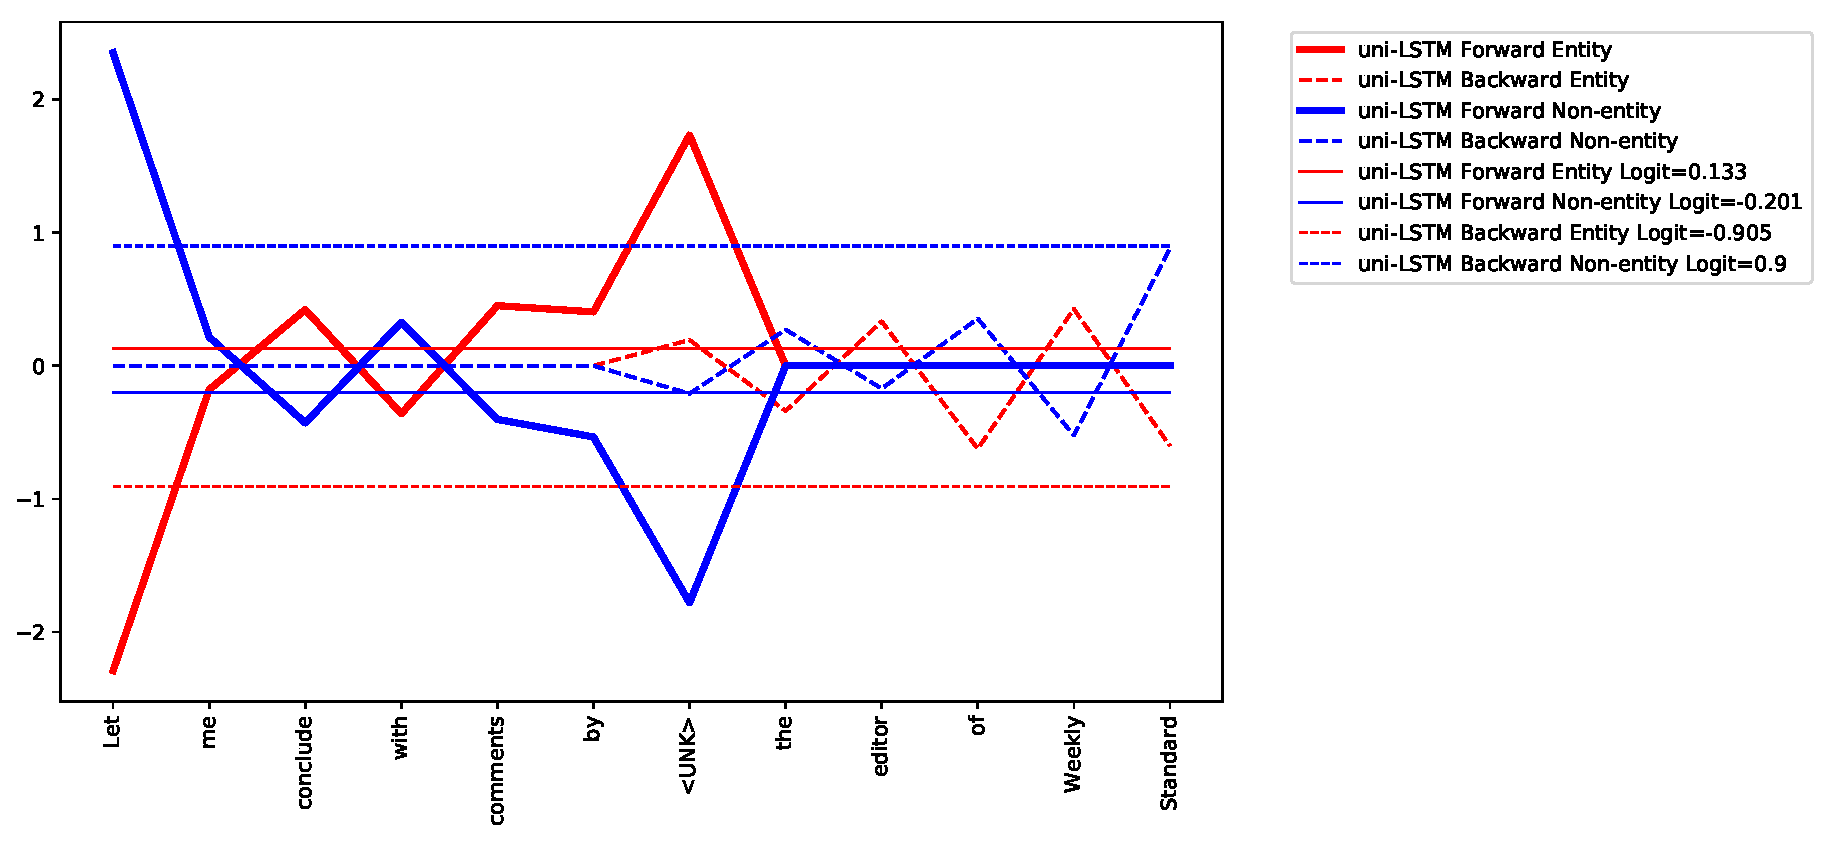
\includegraphics[width=\linewidth]{uni-UNK.pdf}
	\caption{Example 2 for LSTM decomposition contributions to ``$<$UNK$>$''. The x-axis represents token id $j$, and the y-axis represents $\log \beta_{t, j, c}$}
	\label{fig:unk}
\end{figure}

After the replacement, an interesting thing happened. Model in two direction give different prediction: the forward model predict it as entity while the backward model predict it as non-entity. You can see the main contribution to forward model entity prediction still lies in the token position. Since ``$<$UNK$>$'' is a word that can be both entity or non-entity, we conclude that the model learned contextual information from the previous tokens. That is to say, there usually are entities after the word 
``by''. On the other hand, the backward model don't see any special pattern that will predict the token as an entity, so the non-entity pattern is also reasonable. 


\section{Conclusion}

%Can your new technique effectively tackle the problem?
%What future research do you recommend?

\nocite{*}

\bibliographystyle{unsrtnat}

\bibliography{project}

\end{document}